\documentclass[border=4pt]{standalone}
\usepackage{tikz}
\usetikzlibrary{shapes.geometric,positioning,arrows.meta}

\begin{document}
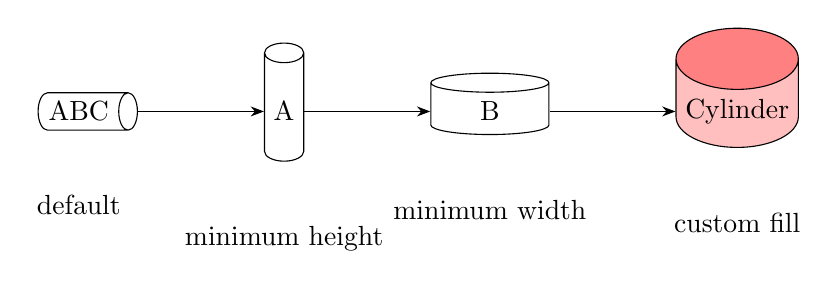
\begin{tikzpicture}[
  >=Stealth,
  every node/.style={cylinder,draw,align=center},
  node distance=1.6cm
]
  \node[shape aspect=.5] (plain) {ABC};
  \node[shape border rotate=90,shape aspect=.5,minimum height=1.5cm,right=of plain] (tall) {A};
  \node[shape border rotate=90,shape aspect=.5,minimum width=1.5cm,right=of tall] (wide) {B};
  \node[
    shape border rotate=90,
    shape aspect=.5,
    cylinder uses custom fill,
    cylinder end fill=red!50,
    cylinder body fill=red!25,
    right=of wide
  ] (filled) {Cylinder};

  \draw[->] (plain.east) -- (tall.west);
  \draw[->] (tall.east) -- (wide.west);
  \draw[->] (wide.east) -- (filled.west);

  \node[draw=none,shape=rectangle,below=7mm of plain] {default};
  \node[draw=none,shape=rectangle,below=7mm of tall] {minimum height};
  \node[draw=none,shape=rectangle,below=7mm of wide] {minimum width};
  \node[draw=none,shape=rectangle,below=7mm of filled] {custom fill};
\end{tikzpicture}
\end{document}
